\documentclass[11pt]{article}
\usepackage[utf8]{inputenc}

\usepackage{geometry}
\geometry{a4paper}

\usepackage{graphicx}
\usepackage{hyperref}
\usepackage[parfill]{parskip}
\usepackage{amsmath, amssymb}
\usepackage{fdsymbol}
\usepackage{color,soul}

% remove section numbering
\makeatletter
\renewcommand{\@seccntformat}[1]{}
\makeatother

% make subsubsection italic
\usepackage{sectsty}
\subsubsectionfont{\itshape}

\renewcommand{\arraystretch}{1.4}

\title{Probability Theory \& Statistics}
\date{}
\author{}

\begin{document}
\maketitle
\clearpage

\section{Interval Estimation}

\subsection{Confidence Intervals}

Suppose \(X_{1}, \ldots, X_{n}\) are random variables with some joint distribution 
depending on a fixed parameter \(\theta\) that may be real or vector-valued.
In previous sessions we have described point estimators of \(\theta\) (see Appendix).

The obvious problem with point estimation is the fact 
that typically \(P_{\theta}(\widehat{\theta} = \theta)\) is small (if not 0) for a given point estimator \(\theta\).
In practice, 
we usually attach to any point estimator an estimator of its variability (for example, its standard error);
however, 
this raises the question of exactly how to interpret such an estimate of variability.

An alternative approach to estimation is interval estimation.
Rather than estimating \(\theta\) by a single statistic, 
we instead give a range of values for \(\theta\) that we feel are consistent 
with observed values of \(X_{1}, \ldots, X_{n}\), 
in the sense, that these parameter values could have produced (with some degree of plausibility) the observed data.

We will start by considering interval estimation for a single (that is, real-valued) parameter.

\emph{Confidence interval}. 
Let \(\boldsymbol{X}=\left(X_{1}, \ldots, X_{n}\right)\) be a vector of random variables with
joint distribution depending on a real-valued parameter \(\theta\) and
let \(L(\boldsymbol{X}) < U(\boldsymbol{X})\) be two statistics. 
Then the (random) interval \(\left[L(\boldsymbol{X}), U(\boldsymbol{X})\right]\) is 
called a \(100p\%\) \emph{confidence interval} for \(\theta\) if
\begin{align}
P_{\theta} \left(L(\boldsymbol{X}) \leq \theta \leq U(\boldsymbol{X})\right) \geq p
\end{align}
for all \(\theta\) with equality for at least one value of \(\theta\).

The number \(p\) is called the \emph{coverage probability} (or simply \emph{coverage}) 
or \emph{confidence level} of the confidence interval. 
In many cases, 
we will be able to find an interval \(\left[L(\boldsymbol{X}), U(\boldsymbol{X})\right]\) with 
\begin{align}
P_{\theta}\left(L(\boldsymbol{X}) \leq \theta \geq U(\boldsymbol{X})\right) = p
\end{align}
for all \(\theta\). 
We can also define upper and lower confidence bounds for \(\theta\). 
For example, 
suppose that
\begin{align}
P_{\theta} \left(\theta \geq L(\boldsymbol{X})\right) = p
\end{align}
for some statistic \(L(\boldsymbol{X})\) and for all \(\theta\); 
then \(L(\boldsymbol{X})\) is called a \(100p\%\) \emph{lower confidence bound} for \(\theta\). 
Likewise, if
\begin{align}
P_{\theta} \left( \theta \leq U(\boldsymbol{X}) \right) = p
\end{align}
for some statistic \(U(\boldsymbol{X})\) and all \(\theta\) 
then \(U(\boldsymbol{X})\) is called a \(100p\%\) \emph{upper confidence bound} for \(\theta\). 

It is easy to see that if \(L(\boldsymbol{X})\) is a \(100p_{1}\%\) lower confidence bound, 
and \(U(\boldsymbol{X})\) is a \(100p_{2}\%\) upper confidence bound for \(\theta\), 
then the interval \(\left[L(\boldsymbol{X}), U(\boldsymbol{X})\right]\) 
is a \(100p\%\) confidence interval for \(\theta\) where \(p = p_{1} + p_{2} - 1\) 
(provided that \(L(\boldsymbol{X}) < U(\boldsymbol{X})\)).

The interpretation of confidence intervals is frequently misunderstood. 
Much of the confusion stems from the fact that confidence intervals are defined in terms of 
the distribution of \(\boldsymbol{X}=\left(X_{1}, \ldots, X_{n}\right)\) but, 
in practice, 
are stated in terms of the observed values of these random variables 
leaving the impression that a probability statement is being made about \(\theta\) rather than about the random interval.

However, 
given data \(X = x\), 
the interval \(\left[L(\boldsymbol{X}), U(\boldsymbol{X})\right]\) will either
contain the true value of \(\theta\) or will not contain the true value of \(\theta\); 
under repeated sampling, 
\(100p\%\) of these intervals will contain the true value of \(\theta\). 
This distinction is important but poorly understood by many non-statisticians.

In many problems, 
it is difficult or impossible to find an exact confidence interval; 
this is particularly true if a model is not completely specified. 
However, it may be possible to find an interval \(\left[L(\boldsymbol{X}), U(\boldsymbol{X})\right]\)
for which 
\begin{align}
P_{\theta} \left(L(\boldsymbol{X}) \leq \theta \leq U(\boldsymbol{X})\right) \approx p,
\end{align}
in which case the resulting interval is called an \emph{approximate} \(100p\%\)
\emph{confidence interval} for \(\theta\).

\subsection{Example}

Suppose that \(X_{1}, \ldots, X_{n}\) are i.i.d. Normal
random variables with mean \(\mu\) and variance 1. 
Then \(\sqrt{n}(\widehat{X} - \mu) \sim N(0,1)\) and so
\begin{align}\label{eq:standard}
P_{\mu}\left(-1.96 \leq \sqrt{n}(\widehat{X} - \mu) \leq 1.96 \right) = 0.95.
\end{align}
The event \(\{-1.96 \leq \sqrt{n}(\widehat{X} - \mu) \leq 1.96 \}\) is clearly 
the same as the event \(\{\widehat{X} - 1.96 / \sqrt{n} \leq \mu \leq \widehat{X} + 1.96 / \sqrt{n} \}\)
and so we have
\begin{align}
P_{\mu}\left(\widehat{X} - \frac{1.96}{\sqrt{n}} \leq \mu \leq \widehat{X} + \frac{1.96}{\sqrt{n}} \right) = 0.95.
\end{align}
Thus the interval whose endpoints are \(\widehat{X} \pm 1.96/\sqrt{n}\)
is a \emph{95\% confidence interval for \(\mu\)}.

Note in this example, 
if we assume only that \(X_{1}, \ldots, X_{n}\) are i.i.d.
with mean \(\mu\) and variance 1 (not necessarily normally distributed),
we have (by the CLT),
\begin{align}
P_{\mu}\left(-1.96 \leq \sqrt{n}(\widehat{X} - \mu) \leq 1.96 \right) \approx 0.95.
\end{align}
if \(n\) is sufficiently large. 
Using the same argument used above, 
it follows that the interval whose endpoints are \(\widehat{X} \pm 1.96/\sqrt{n}\) 
is an \emph{approximate 95\% confidence interval for \(\mu\)}.

\subsection{Interpretation}

Confidence intervals and levels are frequently misunderstood, 
and published studies have shown that even professional scientists often misinterpret them.
\begin{itemize}
\item A 95\% confidence level \emph{does not mean} that for a given realized interval there is a 95\% probability 
that the population parameter lies within the interval (i.e., a 95\% probability that the interval covers the population parameter).
According to the frequentist interpretation, 
once an interval is calculated, 
this interval either covers the parameter value or it does not; 
it is no longer a matter of probability. 
The 95\% probability relates to the reliability of the estimation procedure, 
not to a specific calculated interval.
\item A 95\% confidence level \emph{does not mean} that 95\% of the sample data lie within the confidence interval.
\item A 95\% confidence level \emph{does not mean} that there is a 95\% probability of the parameter 
estimate from a repeat of the experiment falling within the confidence interval computed from a given experiment
\end{itemize}

\begin{figure}[h!]
\centering
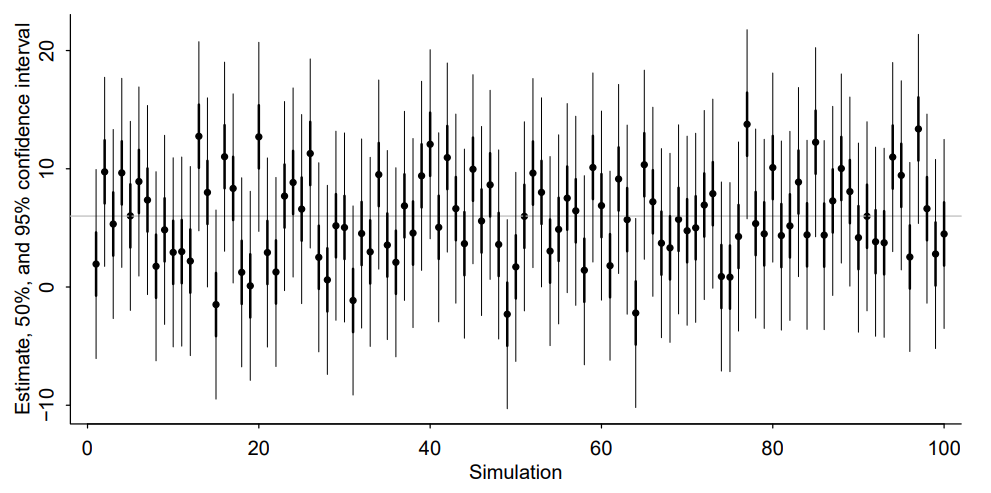
\includegraphics[width=0.75\linewidth]{figure1.png}
\caption{%
Simulation of coverage of confidence intervals: the horizontal line shows the true parameter value,
and dots and vertical lines show estimates and confidence intervals obtained from 100 random simulations from
the sampling distribution. 
If the model is correct, 50\% of the 50\% intervals and 95\% of the 95\% intervals should
contain the true parameter value, in the long run.}
\label{fig:interval}
\end{figure}

A confidence interval can be interpreted as follows (taking the 95\% confidence interval as an example in the following).
\begin{itemize}
\item The confidence interval can be expressed in terms of a long-run 
frequency in repeated samples (or in resampling): \emph{were this procedure to be repeated on numerous samples, 
the proportion of calculated 95\% confidence intervals that encompassed the true value of the population parameter would tend toward 95\%.}
\item The confidence interval can be expressed in terms of probability with respect to a single theoretical (yet to be realized) sample: \emph{there is a 95\% probability that the 95\% confidence interval calculated from a given future sample 
will cover the true value of the population parameter.}
This essentially reframes the repeated samples interpretation as a probability rather than a frequency.
\item The confidence interval can be expressed in terms of statistical significance, e.g.: \emph{the 95\% confidence 
interval represents values that are not statistically significantly different from the point estimate at the .05 level.}
\end{itemize}

\subsection{Counterexample}

Since confidence interval theory was proposed, 
a number of counter-examples to the theory have been developed to show how 
the interpretation of confidence intervals can be problematic, 
at least if one interprets them naïvely.

Suppose that \(X_{1}\) and \(X_{2}\) are independent observations from a uniform \((\theta - 1/2, \theta + 1/2)\) distribution. 
Then the optimal 50\% confidence procedure for \(\theta\) is then
\begin{align}
  \widehat{X}\pm
  \begin{cases}
    \frac{|X_1 - X_2|}{2}, & \text{if $|X_1 - X_2|< 1/2$}\\
    \frac{1 - |X_1 - X_2|}{2}, & \text{if $|X_1 - X_2| \geq 1/2$}.
  \end{cases}
\end{align}
A fiducial or objective Bayesian argument can be used to derive the interval estimate
\begin{align}
  \widehat{X}\pm \frac{|X_1 - X_2|}{4},
\end{align}
which is also a 50\% confidence procedure. 
for every \(\theta_1 \neq \theta\),
the probability that the first procedure contains \(\theta_1\) 
is \emph{less than or equal} to the probability that the second procedure contains \(\theta_1\) .
The average width of the intervals from the first procedure is less than that of the second. 
Hence, the first procedure is preferred under classical confidence interval theory.

However, when \(|X_1 - X_2| \geq 1/2\),
intervals from the first procedure are guaranteed to contain the true value \(\theta\).
Therefore, the nominal 50\% confidence coefficient is unrelated to the uncertainty we should have 
that a specific interval contains the true value. 
The second procedure does not have this property.

Moreover, when the first procedure generates a very short interval, 
this indicates that \(X_{1}\) and \(X_{2}\) are very close together and 
hence only offer the information in a single data point. 
Yet the first interval will exclude almost all reasonable values of the parameter due to its short width. 
The second procedure does not have this property.

The two counter-intuitive properties of the first procedure 
-- 100\% coverage when \(X_{1}\) and \(X_{2}\) are far apart 
and almost 0\% coverage when \(X_{1}\) and \(X_{2}\) are close together 
-- balance out to yield 50\% coverage on average. 
However,
despite the first procedure being optimal, 
its intervals offer neither an assessment of the precision of the estimate 
nor an assessment of the uncertainty one should have that the interval contains the true value.

This counter-example is used to argue against naïve interpretations of confidence intervals. 
If a confidence procedure is asserted to have properties beyond that of the nominal coverage (such as relation to precision, 
or a relationship with Bayesian inference), 
those properties must be proved; 
\emph{they do not follow from the fact that a procedure is a confidence procedure.}

\clearpage
\subsection{Practice}

1) Show Equation \ref{eq:standard} is true for the random variable \(Z \sim N(0,1)\).


\end{document}
